\section{Hungarian Notation for J}\label{ap:jodhung}
   
\begin{figure}[htbp]
  \centering
  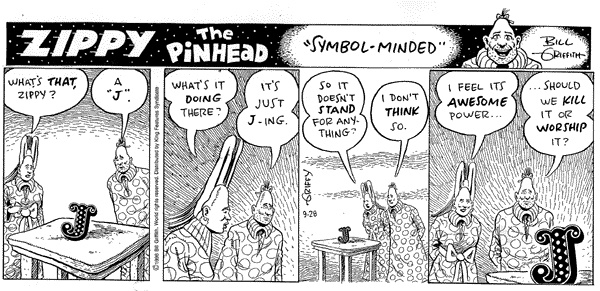
\includegraphics[width=0.8\textwidth]{zippy}
  \caption[Zippy the Pinhead]{Zippy\index{Zippy} \cite{zippy} isn't the only one challenged by the \emph{awesome power} of J.}
  \label{eps:zippy}
\end{figure}

\subsection{Whither Hungarian}

J is a \emph{dynamically typed} language!  What this means is that
you do not have to declare the types of arguments and that types
can change during program execution.  Discarding the 
type declaration machinery found in other programming languages simplifies
J coding but it can impose its own problems. Without declarations
it's not always clear \emph{what is a valid argument}.  J does
not require that you provide hints and, in J's \emph{tacit} case, it
does not even require that you provide arguments!  Given
the language's terse nature this quickly leads to an incomprehensible
style that J detractors have dubbed \emph{line noise}. 

To distinguish my J code from line noise I have adapted a documentation
style known as \href{http://en.wikipedia.org/wiki/Hungarian_notation}{Hungarian notation} \cite{wiki:hung}. 
 Hungarian notation inspires devotion and disgust.  Many swear by it and many
 swear at it.  For me a
convention is worthwhile if it \emph{helps me} understand code.  The style
outlined here helps me understand and maintain J code.  It might help you too.

\subsection{J Noun Types}

There are two broad classes of arguments in J: nouns and verbs.  Nouns are data;
they correspond to arguments found in other programming languages.  Verbs are programs.  J adverbs
and conjunctions take verb arguments.\footnote{Adverbs and conjunctions also take noun
arguments.} Adverbs and conjunctions roughly correspond to the
higher order functions found in languages like
\href{http://www.cs.cmu.edu/Groups/AI/html/cltl/cltl2.html}{\texttt{LISP}} \cite{commonlisp} and
\href{http://www-swiss.ai.mit.edu/projects/scheme/}{\texttt{Scheme}} \cite{scheme}. 
J \emph{explicit} definition syntax reserves the characters \texttt{x y m n
u v} for arguments: see Table~\ref{tab:jargs} on page~\pageref{tab:jargs}.\footnote{
Earlier versions of J used  \texttt{ x.\ y.\ m.\ n.\ u.\ v.\ } for arguments.  This inflected
syntax has been deprecated.} The Hungarian notation described here focuses on noun arguments, 
(\texttt{x} and \texttt{y}), because they are the most common.

\begin{table}[htbp]
  \centering
   \scriptsize
\begin{tabular}{|l|l|} \hline
   \multicolumn{2}{|c|}{\textbf{\normalsize J Explicit Arguments\T\B}} \\ \hline
   \texttt{x\T\B} & \textcolor{CodeComment}{\ttfamily\textsl{left verb noun argument}}  \\
   \texttt{y\T\B} & \textcolor{CodeComment}{\ttfamily\textsl{right verb noun argument}} \\ 
   \texttt{m\T\B} & \textcolor{CodeComment}{\ttfamily\textsl{left conjunction noun argument}} \\ 
   \texttt{n\T\B} & \textcolor{CodeComment}{\ttfamily\textsl{right conjunction noun argument}} \\ 
   \texttt{u\T\B} & \textcolor{CodeComment}{\ttfamily\textsl{left adverb/conjunction verb argument}} \\ 
   \texttt{v\T\B} & \textcolor{CodeComment}{\ttfamily\textsl{right conjunction verb argument}}  \\ \hline
\end{tabular}
   \caption[J Arguments]{Characters reserved for J \emph{explicit} definition arguments. \emph{Tacit} definitions do
   not directly refer to arguments.}
   \label{tab:jargs}
\end{table}

To succinctly describe a J noun you need to be mindful of:
\begin{itemize}
	\item Type
	\item Rank
	\item Boxing
\end{itemize}

\textbf{J types} are congruent to simple types in other languages.  The standard J utility verb \texttt{datatype} enumerates primitive J noun types.

\begin{lstlisting}[frame=single,framerule=0pt,basicstyle=\ttfamily\footnotesize] 
datatype=: 3 : 0
  n=. 1 2 4 8 16 32 64 128 1024 2048 4096 8192 16384 32768 65536 131072
  t=. '/boolean/literal/integer/floating/complex/boxed/extended/rational'
  t=. t,'/sparse boolean/sparse literal/sparse integer/sparse floating'
  t=. t,'/sparse complex/sparse boxed/symbol/unicode'
  (n i. 3!:0 y) pick <;._1 t
)

  NB. types of list items
  datatype&.> (2x^128);1;'char';(s: ' symbol minded');7 %~ i. 4 5
+--------+-------+-------+------+--------+
|extended|boolean|literal|symbol|floating|
+--------+-------+-------+------+--------+
\end{lstlisting}  

\textbf{Rank} has a precise technical meaning in J but in this context it can be loosely
thought of as array dimension.   Typical ranks in J are:
\begin{itemize}
	\item Single numbers like \texttt{42} and characters \texttt{'a'} are called atoms. They
	have \textsl{rank 0}.\footnote{\textsl{Rank 0}, or \textsl{0-dimensional} objects occur in
	in all programming languages but are \emph{rarely recognized.} This leads to mountains of ugly special case code. J is more than a programming language; it's a comprehensive and rigorous way 
to \emph{think} about arrays.} 
	\item Lists like \verb|1 2 3| and \verb|'characters'| correspond to \textsl{1-dimensional} arrays
	in most languages and have \textsl{rank 1}.
	\item Tables like \verb|i. 3 2| are \textsl{2-dimensional} arrays and have \textsl{rank 2}.  
	\item $n$ dimensional arrays have rank $n$.
\end{itemize}

\textbf{Boxing} is structural.  J nouns are either boxed or simple.  A  simple noun
has one of the types, (excluding boxed), listed by
the \texttt{datatype} verb.  To mix types in a J array you must box.
\begin{lstlisting}[frame=single,framerule=0pt] 
      NB. you must box < to mix types in J arrays
      (<u: 'unicode me'),(<i. 2 3),<'types to mix'
\end{lstlisting}  

\subsection{Hungarian Noun Descriptions}

To describe J nouns I use the following rules:\footnote{As in
the film \emph{Pirates of the Caribbean} these rules are more like \emph{guidelines!}} 

\begin{figure}
  \centering
  \ttfamily
  \scriptsize
  \subfigure[J native type prefixes]{
\begin{tabular}{|l|l|l|} \hline
   \multicolumn{3}{|c|}{\rmfamily\textbf{\normalsize J Native Type Prefixes\T\B}} \\ \hline
   \multicolumn{1}{|c|}{\rmfamily\textbf{Prefix\T\B}} &
   \multicolumn{1}{|c|}{\rmfamily\textbf{Native Type\T\B}} &
   \multicolumn{1}{|c|}{\rmfamily\textbf{ \texttt{(3!:0)} code\T\B}} \\ \hline
 p\T\B & \textcolor{CodeComment}{\textsl{boolean}}   &      1  \\    
 c\T\B & \textcolor{CodeComment}{\textsl{literal}}   &      2  \\    
 i\T\B & \textcolor{CodeComment}{\textsl{integer}}   &      4  \\    
 f\T\B & \textcolor{CodeComment}{\textsl{floating}}  &      8  \\    
 j\T\B & \textcolor{CodeComment}{\textsl{complex}}   &      16 \\    
 b\T\B & \textcolor{CodeComment}{\textsl{boxed}}    &      32 \\    
 X\T\B & \textcolor{CodeComment}{\textsl{extended}}  &      64 \\    
 R\T\B & \textcolor{CodeComment}{\textsl{rational}}  &      128  \\  
 SP\T\B & \textcolor{CodeComment}{\textsl{sparse boolean}} & 1024  \\ 
 SC\T\B & \textcolor{CodeComment}{\textsl{sparse literal}} &  2048 \\  
 SI\T\B & \textcolor{CodeComment}{\textsl{sparse integer}} &  4096  \\ 
 SF\T\B & \textcolor{CodeComment}{\textsl{sparse floating}} & 8192 \\  
 SJ\T\B & \textcolor{CodeComment}{\textsl{sparse complex}}  & 16384 \\ 
 SB\T\B & \textcolor{CodeComment}{\textsl{sparse boxed}}    & 32768 \\ 
 s\T\B  & \textcolor{CodeComment}{\textsl{symbol}}          & 65536  \\                 
 w\T\B  & \textcolor{CodeComment}{\textsl{unicode}}         & 131072 \\ \hline
\end{tabular}
  }
  \hspace{0.6cm} %\hfill
  \subfigure[Generic prefixes]{
  \begin{tabular}{|l|l|} \hline
   \multicolumn{2}{|c|}{\rmfamily\textbf{\normalsize Generic Prefixes\T\B}} \\ \hline
   \multicolumn{1}{|c|}{\rmfamily\textbf{Prefix\T\B}} &
   \multicolumn{1}{|c|}{\rmfamily\textbf{Description \T\B}} \\ \hline
 n\T\B & \textcolor{CodeComment}{\textsl{any numeric type including boolean}}  \\   
 N\T\B & \textcolor{CodeComment}{\textsl{any extended numeric type}}  \\
 u\T\B & \textcolor{CodeComment}{\textsl{universal - any J type}}  \\    
 z\T\B & \textcolor{CodeComment}{\textsl{empty - has at least one 0 axis}}  \\ \hline 
\end{tabular}
  }
  \caption[Hungarian Type Prefixes]{\rmfamily Hungarian type prefixes.}
  \label{fig:hungtype}
\end{figure}

\begin{enumerate}
	\item For basic descriptions I use \textsl{TypeRank[Name]}  where \textsl{Type} comes
	from Figure~\ref{fig:hungtype} on page~\pageref{fig:hungtype}, \textsl{Rank} is one of: 
	\begin{center}
	 \footnotesize
\begin{tabular}{ll}
   \texttt{a} & \textcolor{CodeComment}{\ttfamily\textsl{atom - rank 0}} \\ 
   \texttt{l} & \textcolor{CodeComment}{\ttfamily\textsl{list - rank 1}}  \\
   \texttt{t} & \textcolor{CodeComment}{\ttfamily\textsl{table - rank 2}} \\   
   \texttt{[n]} & \textcolor{CodeComment}{\ttfamily\textsl{general rank $n$}} \\ 
\end{tabular}
\end{center}
and \textsl{Name} is an optional descriptive name.  The \textsl{TypeRank} prefix uses
the case of Figure~\ref{fig:hungtype} on page~\pageref{fig:hungtype} and \textsl{Name} begins with an uppercase letter.
 \begin{center}
 \footnotesize
\begin{tabular}{ll}
   \texttt{paSwitch} & \textcolor{CodeComment}{\ttfamily\textsl{boolean (proposition) Switch}} \\ 
   \texttt{ilColors} & \textcolor{CodeComment}{\ttfamily\textsl{integer list Colors}}  \\
   \texttt{ctDocument} & \textcolor{CodeComment}{\ttfamily\textsl{character table Document}} \\   
   \texttt{jt} & \textcolor{CodeComment}{\ttfamily\textsl{complex numerix table or matrix}} \\ 
   \texttt{s[3]Xref} & \textcolor{CodeComment}{\ttfamily\textsl{rank 3 array of Xref symbols}} \\ 
   \texttt{Rl} & \textcolor{CodeComment}{\ttfamily\textsl{extended rational list}} \\ 
   \texttt{bt} & \textcolor{CodeComment}{\ttfamily\textsl{boxed table}} \\
   \texttt{SClRare} & \textcolor{CodeComment}{\ttfamily\textsl{sparse character list Rare}} \\
   \texttt{wlPersian} & \textcolor{CodeComment}{\ttfamily\textsl{unicode list Persian}} \\ 
   \texttt{ztHolder} & \textcolor{CodeComment}{\ttfamily\textsl{empty table Holder}} \\ 
   \texttt{ulWhatever} & \textcolor{CodeComment}{\ttfamily\textsl{universal list - any J list}} \\ 
   \texttt{uu} & \textcolor{CodeComment}{\ttfamily\textsl{universal universal - any J argument}} \\ 
\end{tabular}
\end{center}
 \item For boxed nouns of depth one I use a \textsl{TypeRankTypeRank[Name]} where the right most      pairing describes the boxed types.  Boxed nouns of depth one occur often.
 \begin{center}
 \footnotesize
\begin{tabular}{ll}
   \texttt{blcl} & \textcolor{CodeComment}{\ttfamily\textsl{boxed list of character lists}} \\ 
   \texttt{blit} & \textcolor{CodeComment}{\ttfamily\textsl{boxed list of integer tables}}  \\
   \texttt{bljtCoord} & \textcolor{CodeComment}{\ttfamily\textsl{boxed list of complex tables}} \\   
   \texttt{blul} & \textcolor{CodeComment}{\ttfamily\textsl{boxed list any lists}} \\ 
   \texttt{b[3]s[4]Maps} & \textcolor{CodeComment}{\ttfamily\textsl{boxed rank 3 array of rank 4 symbol array Maps }} \\ 
\end{tabular}
\end{center} 
 \item For more complex nouns, when it's helpful to expose some external structure, I use
 a mixture of more basic noun descriptions and J syntax. 
  \begin{center}
 \footnotesize
\begin{tabular}{ll}
   \texttt{(<blcl),<jtPlane} & \textcolor{CodeComment}{\ttfamily\textsl{two item list}} \\ 
   \texttt{pa;ftXy;<btuu} & \textcolor{CodeComment}{\ttfamily\textsl{three item list}}  \\
   \texttt{cl;ia;(<blcl),<blcl} & 
     \textcolor{CodeComment}{\ttfamily\textsl{see Table~\ref{tab:juses} page~\pageref{tab:juses}}} \\
   \texttt{itYYYYMMDD;slWords;(<bt),<clName} &
     \textcolor{CodeComment}{\ttfamily\textsl{four item list}} \\
   \texttt{saRed,saGreen,saBlue} & 
     \textcolor{CodeComment}{\ttfamily\textsl{emphasize items of simple noun}} \\
\end{tabular} 
\end{center}
 \item Finally, when more than one description is needed I separate individual 
 descriptions with the \emph{or} symbol \argsep and use as many consecutive lines as required.\footnote{The \argsep symbol was chosen because it falls outside 
 of J's ASCII vocabulary and suggests ``either-or.''} 
  \begin{center}
 \footnotesize
\begin{tabular}{l}
 \textcolor{CodeComment}{\ttfamily\textsl{dyadic \hyperlink{il:put}{put} argument description see page~\pageref{ss:put}}} \\
 \texttt{iaObject put clName \argsep blclNames \argsep btNvalues} \\
 \texttt{clLocale put clName \argsep blclNames \argsep btNvalues} \\
 \texttt{(iaObject,iaQualifier) put clName \argsep blclNames}  \\
 \texttt{(iaObject,iaQualifier) put clName btNvalues} \\
 \\
  \textcolor{CodeComment}{\ttfamily\textsl{dyadic \hyperlink{il:dnl}{dnl} argument description see page~\pageref{ss:dnl}}} \\
 \texttt{iaObject dnl zl \argsep clPstr} \\
 \texttt{(iaObject,iaOption) dnl zl \argsep clPstr} \\
  \texttt{(iaObject,iaOption,iaQualifier) dnl zl } \\
  \texttt{(iaObject,iaOption,iaQualifier) dnl clPstr} \\
\end{tabular} 
\end{center}
\end{enumerate}